\section{Player Class Reference}
\label{classPlayer}\index{Player@{Player}}
The same {\bf Monster}{\rm (p.\,\pageref{classMonster})}, but represents human(?) who plays this game.  


{\tt \#include $<$player.hpp$>$}

Inheritance diagram for Player::\begin{figure}[H]
\begin{center}
\leavevmode
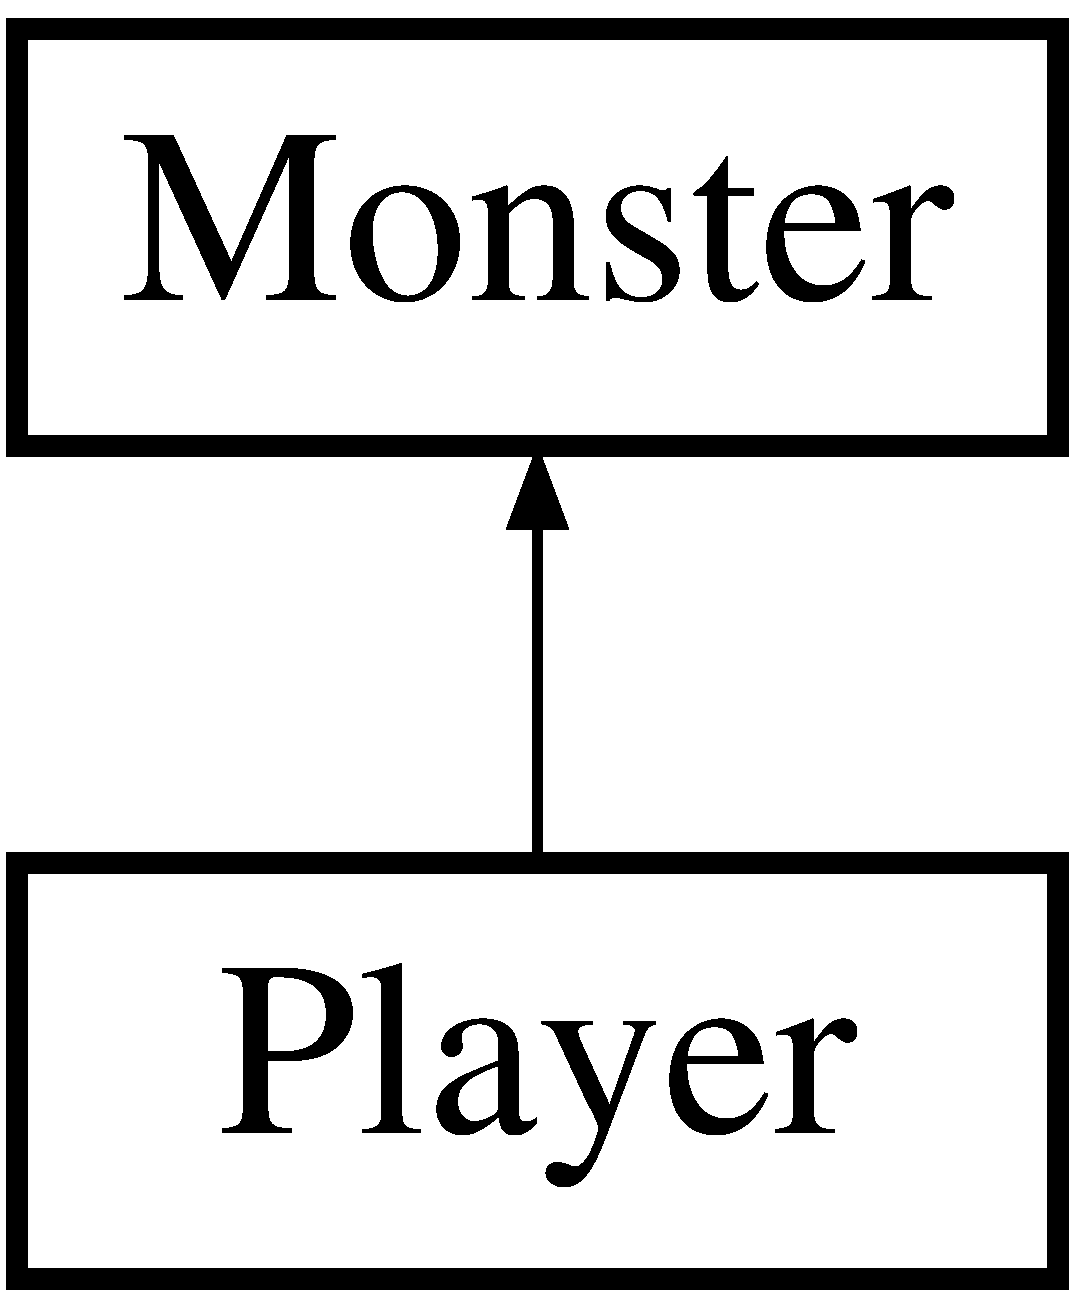
\includegraphics[height=2cm]{classPlayer}
\end{center}
\end{figure}
\subsection*{Signals}
\begin{CompactItemize}
\item 
void {\bf player\-Moved} ()
\item 
void {\bf health\-Change} ()
\end{CompactItemize}
\subsection*{Public Member Functions}
\begin{CompactItemize}
\item 
virtual void {\bf load} ({\bf Parser} \&parser)
\item 
virtual void {\bf save} (ofstream \&file) const 
\item 
virtual bool {\bf is\-Monster} ()
\item 
virtual bool {\bf teleport} (const QString \&{\bf map\-Name}, int {\bf x}, int {\bf y})
\begin{CompactList}\small\item\em Moves monster from it's current map to a map named {\tt map\-Name} at coordinates (x, y). \item\end{CompactList}\item 
virtual void {\bf move\-By} (int dx, int dy)
\item 
virtual void {\bf random} (int {\bf monster\-Type})
\item 
virtual void {\bf reset\-Maximums} ()
\item 
virtual void {\bf naturally\-Regenerate} ()
\item 
virtual void {\bf damaged} ()
\end{CompactItemize}


\subsection{Detailed Description}
The same {\bf Monster}{\rm (p.\,\pageref{classMonster})}, but represents human(?) who plays this game. 



\subsection{Member Function Documentation}
\index{Player@{Player}!damaged@{damaged}}
\index{damaged@{damaged}!Player@{Player}}
\subsubsection{\setlength{\rightskip}{0pt plus 5cm}void damaged ()\hspace{0.3cm}{\tt  [virtual]}}\label{classPlayer_a8}




Reimplemented from {\bf Monster} {\rm (p.\,\pageref{classMonster_a35})}.\index{Player@{Player}!healthChange@{healthChange}}
\index{healthChange@{healthChange}!Player@{Player}}
\subsubsection{\setlength{\rightskip}{0pt plus 5cm}void health\-Change ()\hspace{0.3cm}{\tt  [signal]}}\label{classPlayer_l1}


\index{Player@{Player}!isMonster@{isMonster}}
\index{isMonster@{isMonster}!Player@{Player}}
\subsubsection{\setlength{\rightskip}{0pt plus 5cm}bool is\-Monster ()\hspace{0.3cm}{\tt  [virtual]}}\label{classPlayer_a2}




Reimplemented from {\bf Monster} {\rm (p.\,\pageref{classMonster_a27})}.\index{Player@{Player}!load@{load}}
\index{load@{load}!Player@{Player}}
\subsubsection{\setlength{\rightskip}{0pt plus 5cm}void load ({\bf Parser} \& {\em parser})\hspace{0.3cm}{\tt  [virtual]}}\label{classPlayer_a0}




Reimplemented from {\bf Monster} {\rm (p.\,\pageref{classMonster_a3})}.\index{Player@{Player}!moveBy@{moveBy}}
\index{moveBy@{moveBy}!Player@{Player}}
\subsubsection{\setlength{\rightskip}{0pt plus 5cm}void move\-By (int {\em dx}, int {\em dy})\hspace{0.3cm}{\tt  [virtual]}}\label{classPlayer_a4}




Reimplemented from {\bf Monster} {\rm (p.\,\pageref{classMonster_a33})}.\index{Player@{Player}!naturallyRegenerate@{naturallyRegenerate}}
\index{naturallyRegenerate@{naturallyRegenerate}!Player@{Player}}
\subsubsection{\setlength{\rightskip}{0pt plus 5cm}void naturally\-Regenerate ()\hspace{0.3cm}{\tt  [virtual]}}\label{classPlayer_a7}




Reimplemented from {\bf Monster} {\rm (p.\,\pageref{classMonster_a10})}.\index{Player@{Player}!playerMoved@{playerMoved}}
\index{playerMoved@{playerMoved}!Player@{Player}}
\subsubsection{\setlength{\rightskip}{0pt plus 5cm}void player\-Moved ()\hspace{0.3cm}{\tt  [signal]}}\label{classPlayer_l0}


\index{Player@{Player}!random@{random}}
\index{random@{random}!Player@{Player}}
\subsubsection{\setlength{\rightskip}{0pt plus 5cm}void random (int {\em monster\-Type})\hspace{0.3cm}{\tt  [virtual]}}\label{classPlayer_a5}




Reimplemented from {\bf Monster} {\rm (p.\,\pageref{classMonster_a5})}.\index{Player@{Player}!resetMaximums@{resetMaximums}}
\index{resetMaximums@{resetMaximums}!Player@{Player}}
\subsubsection{\setlength{\rightskip}{0pt plus 5cm}void reset\-Maximums ()\hspace{0.3cm}{\tt  [virtual]}}\label{classPlayer_a6}




Reimplemented from {\bf Monster} {\rm (p.\,\pageref{classMonster_a8})}.\index{Player@{Player}!save@{save}}
\index{save@{save}!Player@{Player}}
\subsubsection{\setlength{\rightskip}{0pt plus 5cm}void save (ofstream \& {\em file}) const\hspace{0.3cm}{\tt  [virtual]}}\label{classPlayer_a1}




Reimplemented from {\bf Monster} {\rm (p.\,\pageref{classMonster_a4})}.\index{Player@{Player}!teleport@{teleport}}
\index{teleport@{teleport}!Player@{Player}}
\subsubsection{\setlength{\rightskip}{0pt plus 5cm}bool teleport (const QString \& {\em map\-Name}, int {\em x}, int {\em y})\hspace{0.3cm}{\tt  [virtual]}}\label{classPlayer_a3}


Moves monster from it's current map to a map named {\tt map\-Name} at coordinates (x, y). 

Doesn't check whether it can be moved here. \begin{Desc}
\item[Returns:]false, if such map or square does not exist\end{Desc}


Reimplemented from {\bf Monster} {\rm (p.\,\pageref{classMonster_a32})}.

The documentation for this class was generated from the following files:\begin{CompactItemize}
\item 
{\bf player.hpp}\item 
{\bf player.cpp}\end{CompactItemize}
